\chapter{Experiments}
In this chapter, the quality of the Network and Tracker modules is characterized. First, the available neural networks will be evaluated with a common tracker to select the final neural network used in the dl-objecttracker application. Second, several trackers implementations will be also characterized using the selected neural network. The configurable parameters will be adjusted to select the best performing values. This will give us the best combination of Network and Tracker modules for the final dl-objecttracker, which will also be experimentally validated.\\
\section{Experimental setup}
The experiments were performed on a laptop PC with \textit{Intel® Core™ i7-4510U CPU @ 2.00GHz x 4} and no GPU acceleration.\\ As commented in section \ref{metrics_tool}, the Object Detection Metrics tool was used to compute the following metrics: precision, recall and AP. It is necessary to mention that the tool was slightly modified to provide the TP, FP and GT numbers. The speed measuremenents are obtained directly from the \texttt{dl-objecttracker} for both the Network and the Tracker modules.\\
The selected dataset for evaluating the tracking application and its modules is the MOT17Det \cite{milan2016mot16} \textit{train} set (see Table \ref{tab:annex_3}). The results were not evaluated on the \textit{test} set due to the fact that the official web of the challenge does not include in the provided data the annotated ground truth of the test set. To obtain the ground truth from this dataset and adapt it to the metrics tool a small Python script was developed in this project following the official reference \cite{milan2016mot16}. However, some modifications were done to allow the compatibility between the metrics tool and the labels of the detections (the neural networks are trained in COCO or PASCAL) (see Table \ref{tab:mot_labels}). Following the official MOT interpretation of ground truth detection files, the final ground truth obtained from the train set only includes the \textit{person} class.
\begin{table}[H]
\scriptsize
\begin{center}
\begin{tabular}{|c|l|l|}
\hline
\textbf{ID}                       & \multicolumn{1}{c|}{\textbf{Label in MOT gt}} & \multicolumn{1}{c|}{\textbf{Label in our gt}} \\ \hline
\textbf{1}                        & Pedestrian                                    & Person                                        \\ \hline
\textbf{2}                        & Person on vehicle                             & Car                                           \\ \hline
\textbf{3}                        & Car                                           & Car                                           \\ \hline
\textbf{4}                        & Bicycle                                       & Bicycle                                       \\ \hline
\textbf{5}                        & Motorbike                                     & Motorbike                                     \\ \hline
\textbf{6}                        & Non motorized vehicle                         & Bicycle                                       \\ \hline
\textbf{7}                        & Static person                                 & Person                                        \\ \hline
\textbf{8}                        & Distractor                                    & -                                             \\ \hline
\textbf{9}                        & Occluder                                      & -                                             \\ \hline
\textbf{10}                       & Occluder on the ground                        & -                                             \\ \hline
\textbf{11}                       & Occluder full                                 & -                                             \\ \hline
\multicolumn{1}{|l|}{\textbf{12}} & Reflection                                    & -                                             \\ \hline
\end{tabular}
\end{center}
\caption{Label equivalences with MOT ground truth in our ground truth}
\label{tab:mot_labels}
\end{table}
\section{Neural network selection}
The correct selection of a neural network model for object detection is crucial in this project as it provides the previous detections the tracker module needs to track. As commented in section \ref{neural_networks}, the avalable neural networks models which have been integrated into dl-objecttracker are:
\begin{itemize}
    \item SSD MobileNetV2, pretrained on COCO (Tensorflow)
    \item Faster R-CNN InceptionV2, pretrained on COCO (Tensorflow)
    \item Mask R-CNN InceptionV2, pretrained on COCO (Tensorflow)
    \item SSD VGG, pretrained on Pascal VOC (Keras)
\end{itemize}
Three sequences from the MOT17Det dataset were selected to evaluate the performance of the models. The reason is that these sequences represent most of the possible difficulties that may appear in multiple object tracking tasks such as occlusions, new targets, fixed camera, big motion from frame to frame, etc. The selected sequences are MOT17-05, MOT17-09 and MOT17-11 (Figure \ref{fig:mot_images})\label{selected_sequences}.\\
\begin{figure}[H]
\begin{center}
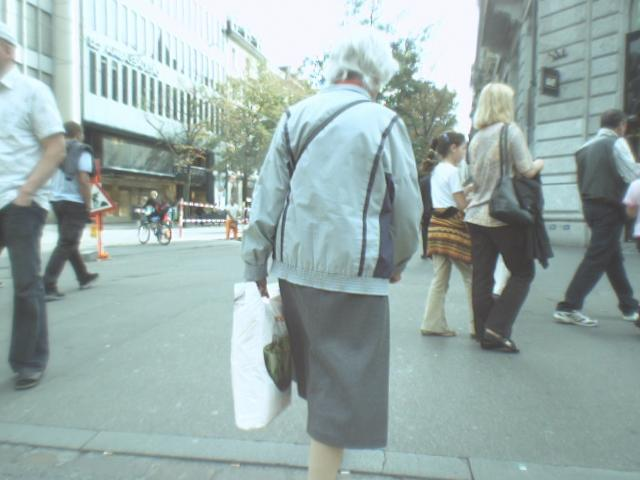
\includegraphics[scale=0.2]{figures/000334.jpg}
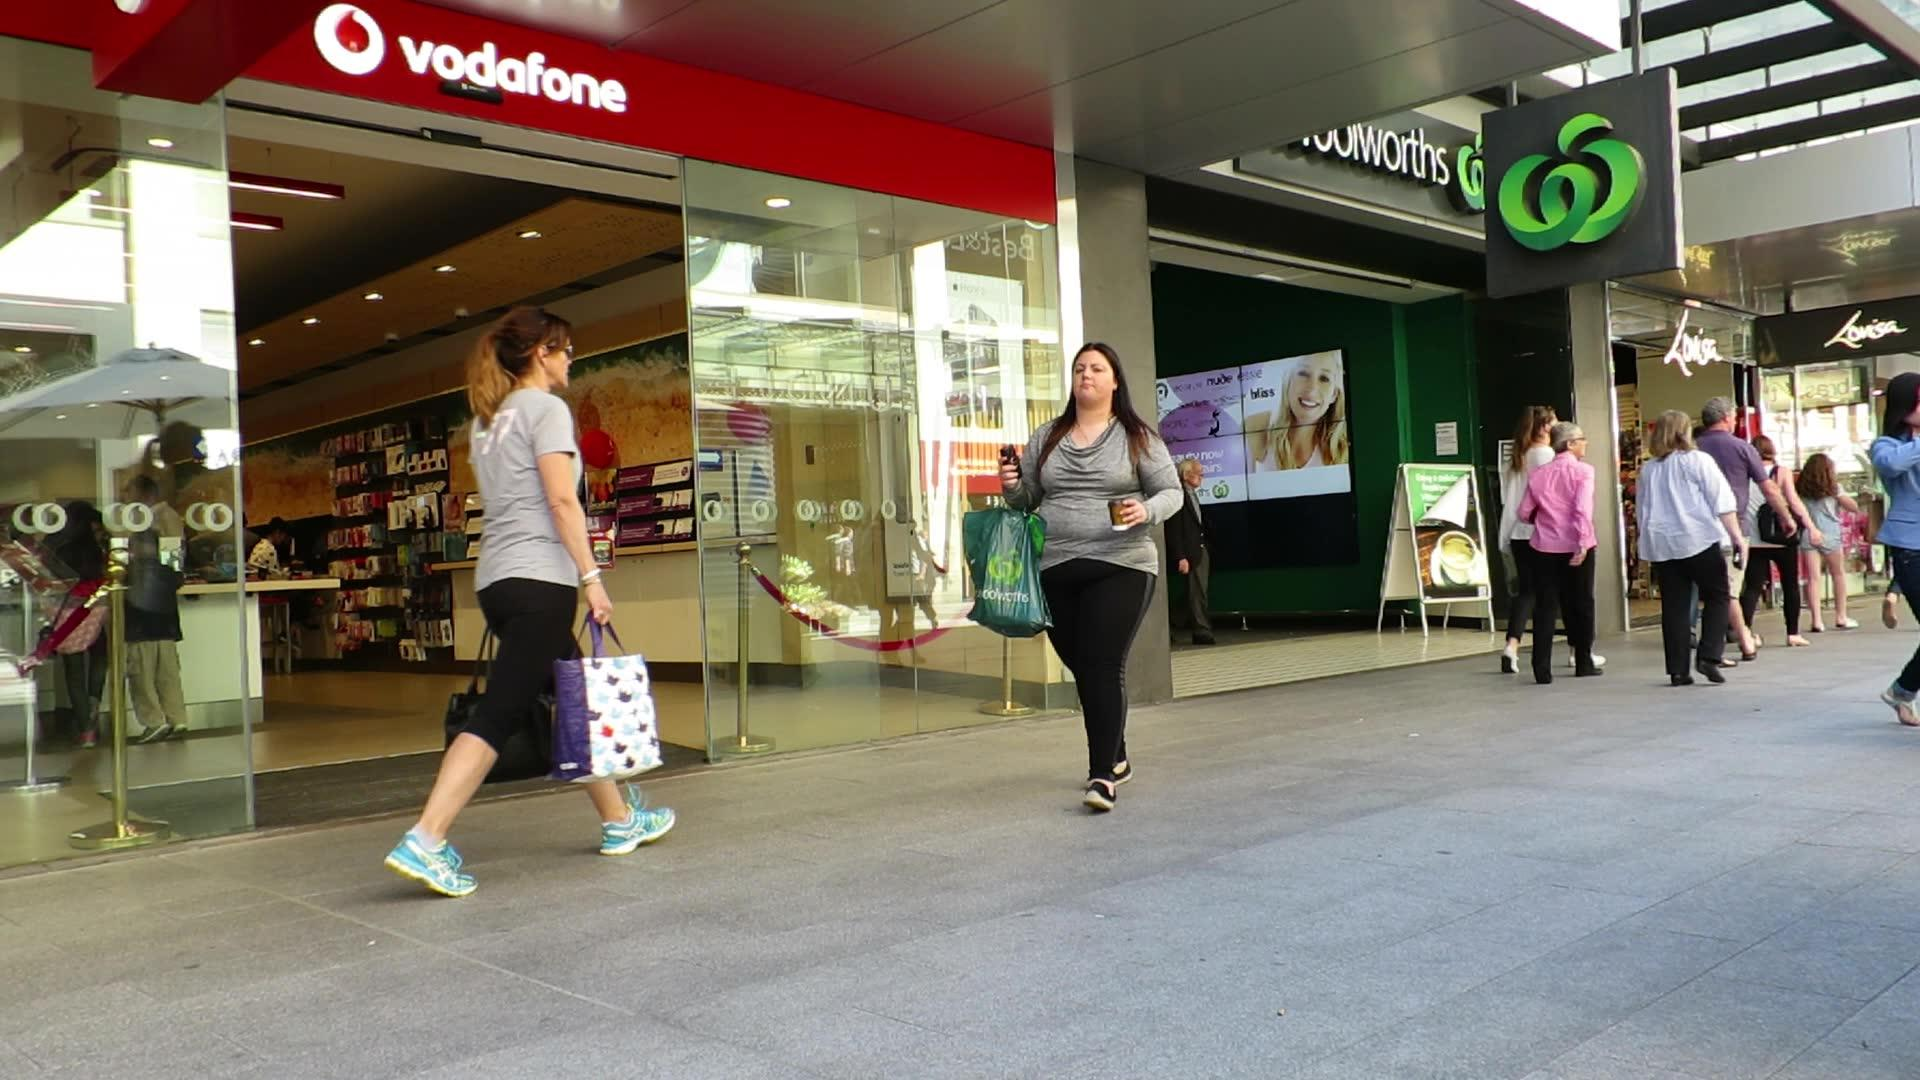
\includegraphics[scale=0.08]{figures/000388.jpg}
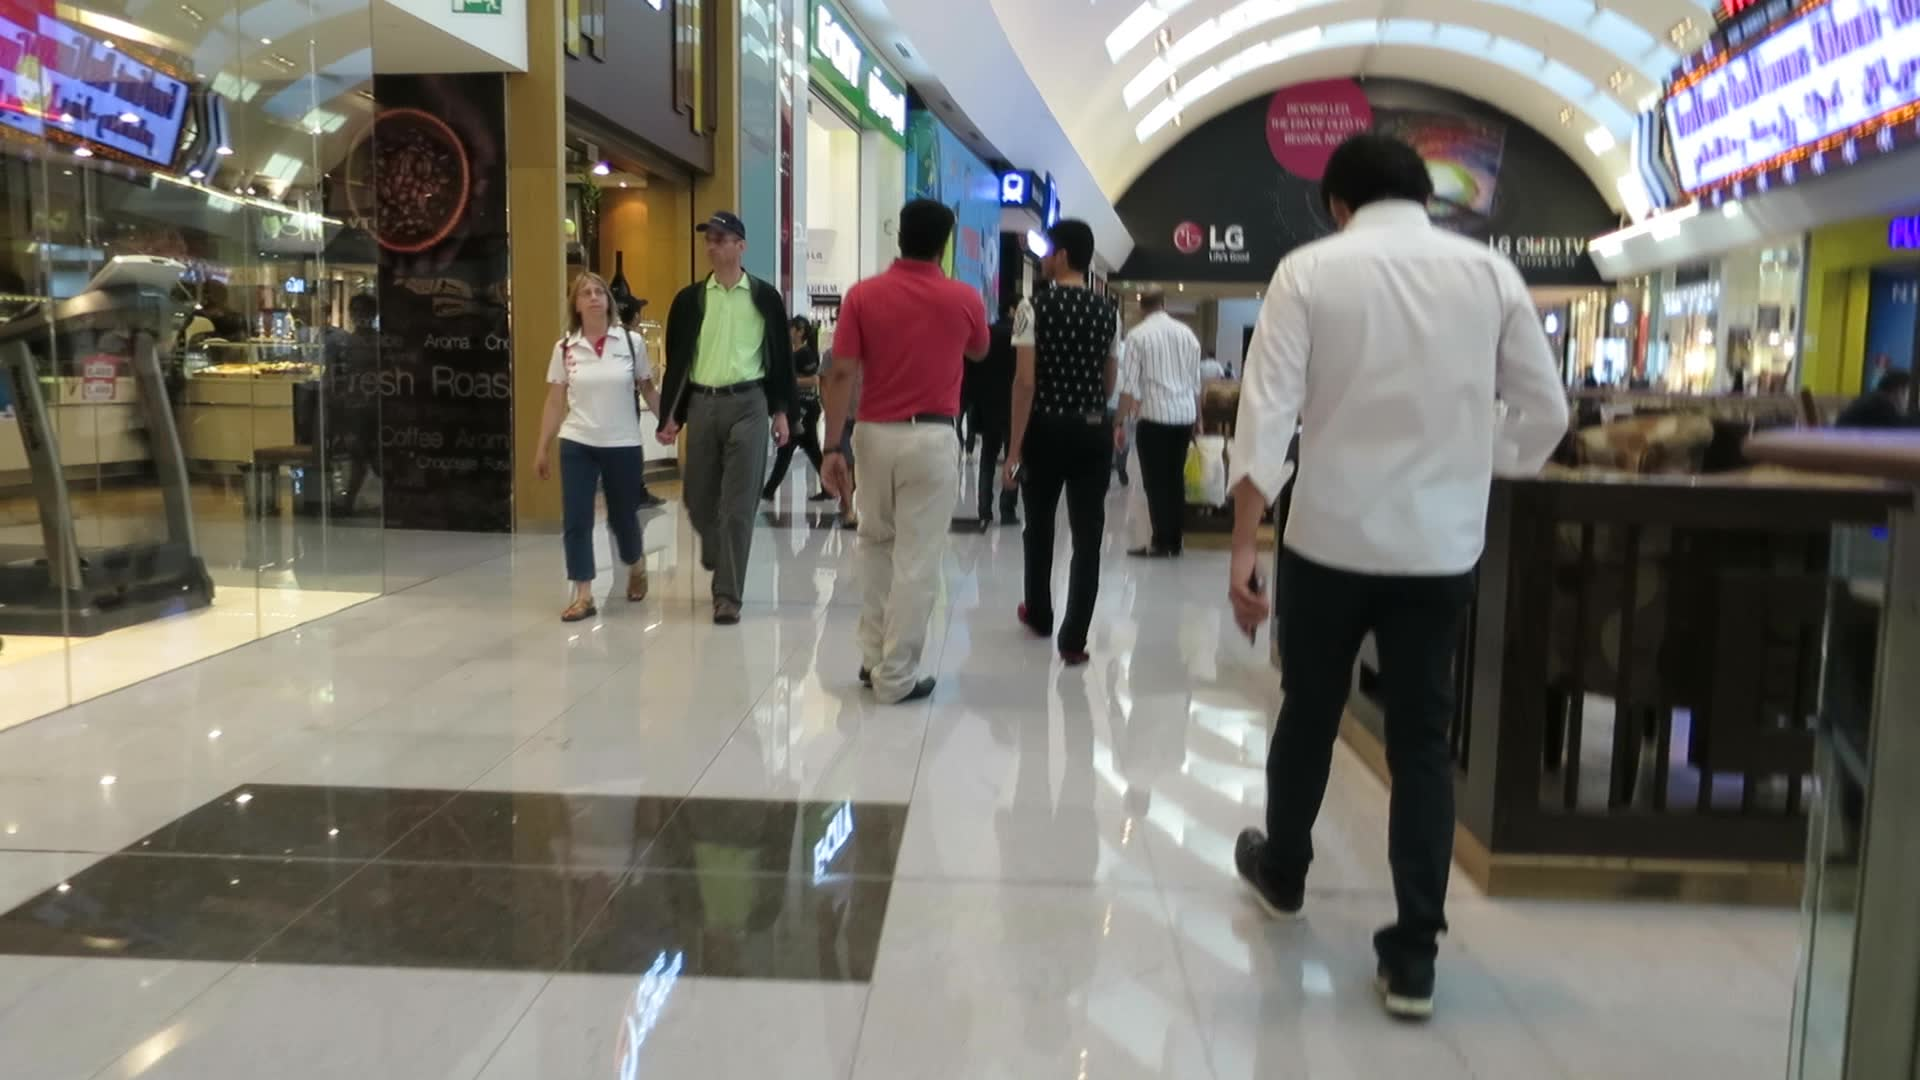
\includegraphics[scale=0.08]{figures/000487.jpg}
\caption{MOT17Det train set samples: left image from MOT17-05, center image from MOT17-09 and right image from MOT17-11}
\label{fig:mot_images}
\end{center}
\end{figure}
The MOSSE tracker was selected as regular tracker and the threshold for all neural network detection was fixed to 0,6. This was done to allow a fair comparison between the models.\\
The MOT17-09 sequence has a fixed camera with several pedestrians walking in groups or alone. In this sequence, the tracking may find fast motion difficulties as well as continuous people coming in and out from the scene. To evaluate the performance in that sequence, two input image sizes were selected due to the Keras SSD-VGG fixed image input size.\\ From the table \ref{tab:net_exp_1}, it can be seen that the maximum AP value is obtained by the Faster R-CNN using 512x512 whereas Mask R-CNN gets the best AP score for 300x300 images. As expected, the R-CNN detectors obtain the best accuracy. However, this accuracy is not linked with the speed in the object detection. The SSD MobileNetV2 gets the best speed rate in both experiments.\\
\begin{table}[H]
\scriptsize
\begin{center}
\begin{tabular}{|c|c|c|}
\hline
\textbf{}                         & \textbf{AP @ 0,5 (\%)} & \textbf{FPS Net} \\ \hline
\textbf{SSD MobileNetV2}          & 16,06                  & 5,282            \\ \hline
\textbf{Faster R-CNN InceptionV2} & 31,03                  & 1,026            \\ \hline
\textbf{Mask R-CNN InceptionV2}   & 27,89                  & 0,286            \\ \hline
\textbf{SSD VGG 512}              & 23,76                  & 0,339            \\ \hline
\end{tabular}
\end{center}
\caption{Experiments on MOT17-09 sequence with 512x512 images}
\label{tab:net_exp_1}
\end{table}
\begin{table}[H]
\scriptsize
\begin{center}
\begin{tabular}{|c|c|c|}
\hline
\textbf{}                         & \textbf{AP @ 0,5 (\%)} & \textbf{FPS Net} \\ \hline
\textbf{SSD MobileNetV2}          & 11,48                  & 8,25             \\ \hline
\textbf{Faster R-CNN InceptionV2} & 24,36                  & 1,067            \\ \hline
\textbf{Mask R-CNN InceptionV2}   & 26,25                  & 0,292            \\ \hline
\textbf{SSD VGG 300}              & 19,08                  & 0,988            \\ \hline
\end{tabular}
\end{center}
\caption{Experiments on MOT17-09 sequence with 300x300 images}
\label{tab:net_exp_2}
\end{table}
The influence of the image input size in the processing speed and the accuracy of the models is clear. The smaller the input size of the image the faster the detections are obtained. In the opposite way, with a bigger input image the final AP result is better. This trend will be confirmed in following experiments.\\

The SSD-VGG models were discarded from other experiments due to its lack of flexibility about the input image size. In the table \ref{tab:net_exp_3}  it can be observed the different performances for 800x800 images of the region-based object detectors and the single-shot object detectors. As it ocurred with smaller image input sizes, the region-based models have a better AP performance almost doubling the AP obtained by the SSD (in the case of Mask R-CNN). For this reason, the SSD MobileNet V2 was eliminated from the neural net selection procedure despite being the fastest. 
\begin{table}[H]
\scriptsize
\begin{center}
\begin{tabular}{|c|c|c|}
\hline
\textbf{}                         & \textbf{AP @ 0,5 (\%)} & \textbf{FPS Net} \\ \hline
\textbf{SSD MobileNetV2}          & 17,13                  & 7,372             \\ \hline
\textbf{Faster R-CNN InceptionV2} & 32,00                  & 0,981            \\ \hline
\textbf{Mask R-CNN InceptionV2}   & 34,23                  & 0,272            \\ \hline
\end{tabular}
\end{center}
\caption{Experiments with 800x800 images}
\label{tab:net_exp_3}
\end{table}
The final experiments were done with Faster R-CNN and Mask R-CNN in MOT17-09, MOT17-11 and MOT17-05. The last two sequences have a common characteristic which is that the camera is in motion. Thus, the sequences are enumerated in order of increasing degree of motion, starting from MOT-09 to MOT-05.
\begin{table}[H]
\scriptsize
\begin{center}
\begin{tabular}{|c|c|c|c|}
\hline
\textbf{AP @ 0,5 (\%)}            & \textbf{MOT17-09} & \textbf{MOT17-11} & \multicolumn{1}{l|}{\textbf{MOT17-05}} \\ \hline
\textbf{Faster R-CNN InceptionV2} & 35,25             & 26,21             & 19,51                                  \\ \hline
\textbf{Mask R-CNN InceptionV2}   & 31,74             & 26,44             & 12,98                                  \\ \hline
\end{tabular}
\end{center}
\caption{Neural network experiments with an image input size of 1000x1000}
\label{tab:net_exp_4}
\end{table}
From these experiments on table \ref{tab:net_exp_4}, it can be seen that the final average precision is similar in the sequence MOT17-11, however, the use of Faster R-CNN model outperforms Mask R-CNN in the other two sequences. These AP scores can be related with the frame rate obtained from each neural network which is about 0,9 FPS for Faster R-CNN and 0,2 FPS for Mask R-CNN. A higher speed can help the tracking procedure to be ``refreshed" more frequently which may lead to better performance on sequences with varying motion between frames as it occurs on the evaluated sequences.\\ In the figure \ref{fig:faster_dets} it can be observed an example of the detections obtained with Faster R-CNN. Generally, the results seem to be pretty accurate but they include some false positives such as the person assigned to a confidence of the 69\%.\\
Given these cuantitative results, the final neural network chosen to perform the object detection in dl-objecttracker is Faster R-CNN InceptionV2.
\begin{figure}[H]
\begin{center}
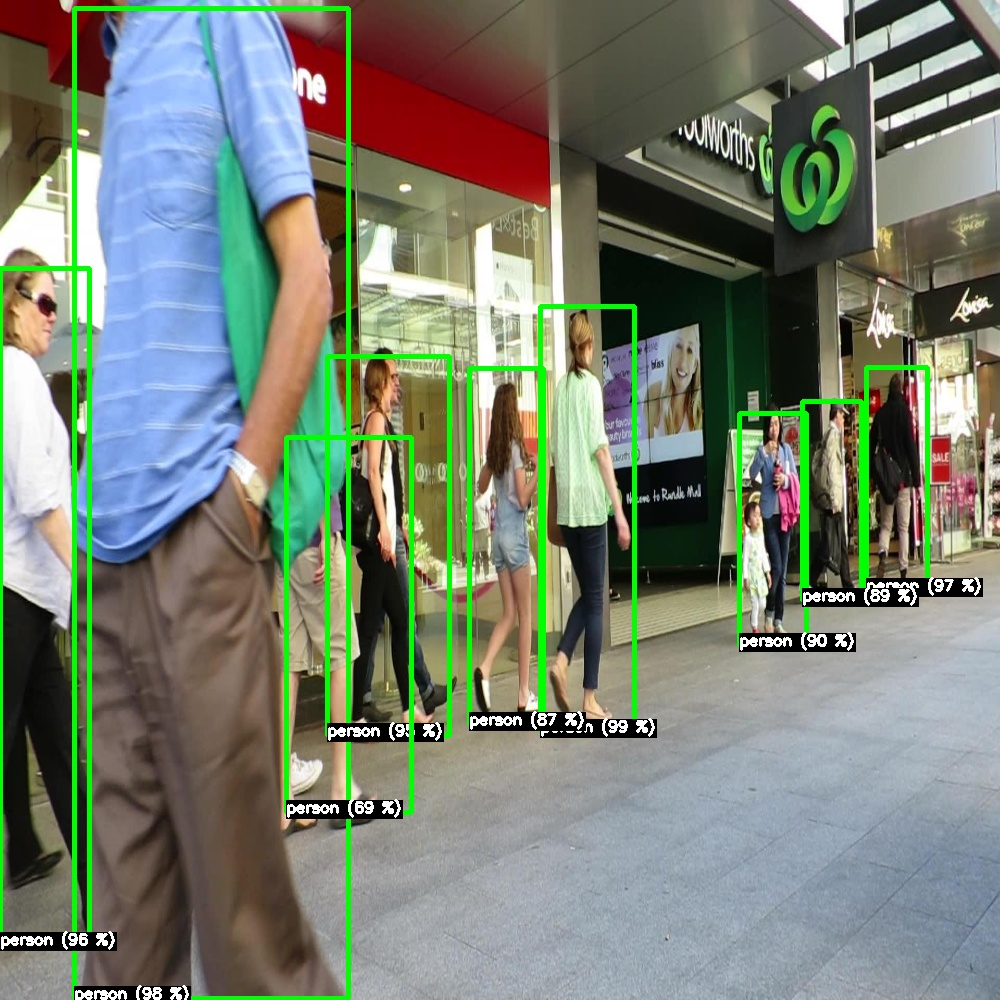
\includegraphics[scale=0.2]{figures/212.jpg}
\caption{Faster R-CNN Inception V2 object detections on MOT17-09}
\label{fig:faster_dets}
\end{center}
\end{figure}
\section{Tracker's performance}
Once the neural network was selected, it is time to evaluate the performance of the second module involved in the core of the multiobject tracking application, the tracking module.\\
The following experiments were done on the same sequences as the Network experiments. In this case, the default configuration includes Faster R-CNN as neural network with a confidence threshold for detection set to 0,6. The confidence of the tracker is being used if no comment is made on it. This confidence is going to be modified later in this section to see its influence on the results. The following tracking algorithms were evaluated: KCF, BOOSTING, MIL, TLD, MEDIANFLOW, CSRT, MOSSE and CF-dlib (section \ref{tracker_algorithms}).\\
\begin{table}[H]
\scriptsize
\begin{center}
\begin{tabular}{|c|c|c|}
\hline
\textbf{}           & \textbf{AP @ 0,5 (\%)} & \textbf{FPS Tracker} \\ \hline
\textbf{KCF}        & \textit{23,07}         & \textit{6,39}        \\ \hline
\textbf{BOOSTING}   & 13,06                  & 4,78                 \\ \hline
\textbf{MIL}        & 15,29                  & 2,21                 \\ \hline
\textbf{TLD}        & 8,38                   & 2,22                 \\ \hline
\textbf{MEDIANFLOW} & \textit{32,13}         & \textit{12,01}       \\ \hline
\textbf{CSRT}       & 11,78                  & 2,78                 \\ \hline
\textbf{MOSSE}      & \textit{34,60}         & \textit{47,07}       \\ \hline
\textbf{CF-dlib}    & \textit{27,99}         & \textit{9,51}        \\ \hline
\end{tabular}
\end{center}
\caption{Tracker experiments on MOT17-09 sequence with 1000x1000 images}
\label{tab:tracker_exp_1}
\end{table}
This experiment provides clear results on the performance of the trackers in the MOT17-09 sequence. The KCF, MEDIANFLOW, MOSSE and CF-dlib outperform in a significant way the accuracy of the rest of the trackers (in terms of AP). A good AP seems to be related with a good frame rate in the tracking.\\
The scheme of evaluating the performance with sequences of increasing difficulty was followed, the second experiment was performed with the MOT17-11 sequence and its results are shown in table \ref{tab:tracker_exp_2}.

\begin{table}[H]
\scriptsize
\begin{center}
\begin{tabular}{|c|c|c|}
\hline
\textbf{}           & \textbf{AP @ 0,5 (\%)} & \textbf{FPS Tracker} \\ \hline
\textbf{KCF}        & 19,17                  & 4,7                  \\ \hline
\textbf{MEDIANFLOW} & \textit{27,76}         & \textit{12,88}       \\ \hline
\textbf{MOSSE}      & \textit{26,23}         & \textit{33,56}       \\ \hline
\textbf{CF-dlib}    & \textit{25,49}         & \textit{9,95}        \\ \hline
\end{tabular}
\end{center}
\caption{Tracker experiments on MOT17-11 sequence with 1000x1000 images}
\label{tab:tracker_exp_2}
\end{table}
The results in this sequence seem to indicate that the KCF tracker is not adecuated for the task. Its results in both AP and the speed measurements are below the overall average.
\begin{table}[H]
\scriptsize
\begin{center}
\begin{tabular}{|c|c|c|}
\hline
\textbf{}           & \textbf{AP @ 0,5 (\%)} & \textbf{FPS Tracker} \\ \hline
\textbf{MEDIANFLOW} & \textit{24,01}         & \textit{13,05}       \\ \hline
\textbf{MOSSE}      & 16,15                  & 18,14               \\ \hline
\textbf{CF-dlib}    & 23,97                  & 9,51                 \\ \hline
\end{tabular}
\end{center}
\caption{Tracker experiments on MOT17-05 sequence with 1000x1000 images}
\label{tab:tracker_exp_3}
\end{table}
The results from table \ref{tab:tracker_exp_2} led us to three final tracker options: MEDIANFLOW, MOSSE and CF-dlib. In the experiment on MOT17-05 shown on table \ref{tab:tracker_exp_3}, MEDIANFLOW gets the overall best performance. It achieves the highest AP score of the three tracker options and the second faster tracking. The faster tracker is MOSSE, following the trend of previous experiments.
\subsection{Confidence in tracking}
In section \ref{conf_in_tracking}, the mechanism of confidence of the tracker was introduced. The tracker itself continuously checks if the tracking obtained for each object is reliable enough. In this section, the importance of this parameter is going to be evaluated. To do so, the performance of the three best tracking algorithms is measured when the confidence is taken into account and in the opposite case. The selected sequences are MOT17-05 and MOT17-09 with a frame size of 500x500 and the neural network used in both cases is Faster R-CNN InceptionV2.\\
\begin{table}[H]
\scriptsize
\begin{center}
\begin{tabular}{|c|c|c|}
\hline
\textbf{}           & \textbf{AP tracker on @ 0,5 (\%)} & \textbf{AP tracker off @ 0,5 (\%)} \\ \hline
\textbf{MEDIANFLOW} & 36,09                             & 32,35                              \\ \hline
\textbf{MOSSE}      & 18,60                             & 10,33                              \\ \hline
\textbf{CF-dlib}    & 23,74                             & 30,06                              \\ \hline
\end{tabular}
\end{center}
\caption{Confidence influence on tracking performance on MOT17-05}
\label{tab:tracker_exp_4}
\end{table}
\begin{table}[H]
\scriptsize
\begin{center}
\begin{tabular}{|c|c|c|}
\hline
\textbf{}           & \textbf{AP tracker on @ 0,5 (\%)} & \textbf{AP tracker off @ 0,5 (\%)} \\ \hline
\textbf{MEDIANFLOW} & 37,80                             & 36,17                              \\ \hline
\textbf{MOSSE}      & 30,16                             & 21,83                              \\ \hline
\textbf{CF-dlib}    & 28,06                             & 31,60                              \\ \hline
\end{tabular}
\end{center}
\caption{Confidence influence on tracking performance on MOT17-09}
\label{tab:tracker_exp_5}
\end{table}
In the tables \ref{tab:tracker_exp_4} and \ref{tab:tracker_exp_5} the results seem to indicate that the influence of taking into account the confidence parameter with OpenCV trackers is positive. However, it occurs the opposite for the \texttt{dlib} tracking with CF.\\
The MEDIANFLOW tracker was finally selected to perform the tracking in the dl-objecttracker application given the performace shown in the previous experiments. Figure \ref{fig:medianflow_images} shows an example of the tracking using that tracking algorithm.\\
Finally, the image input size was modified to check which size was best appropriate to our problem. In table \ref{tab:annex_1} of the \textit{Annex}, the image size of 400x400 gets the best balance between speed and accuracy for the tracking task. Given the tracker and the image size, the threshold for the confidence of the detections from the object detection neural networks was evaluated. Using values ranging from 0,3 to 0,7 the experimental threshold selected was 0,5.
\begin{figure}[H]
\begin{center}
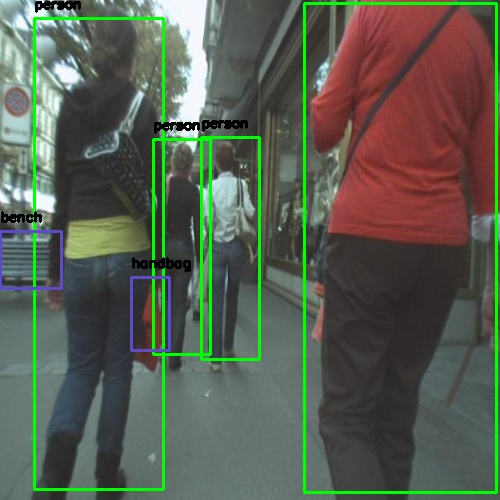
\includegraphics[scale=0.25]{figures/652.jpg}
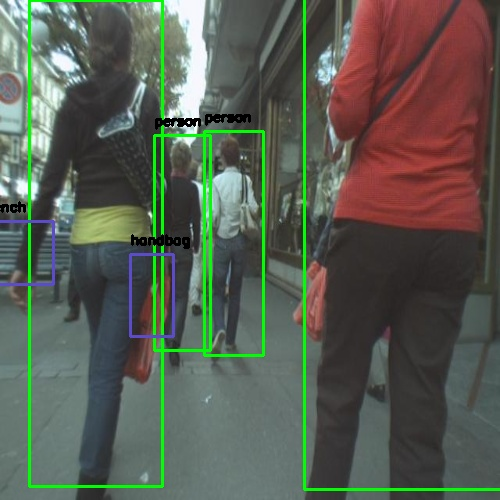
\includegraphics[scale=0.25]{figures/655.jpg}
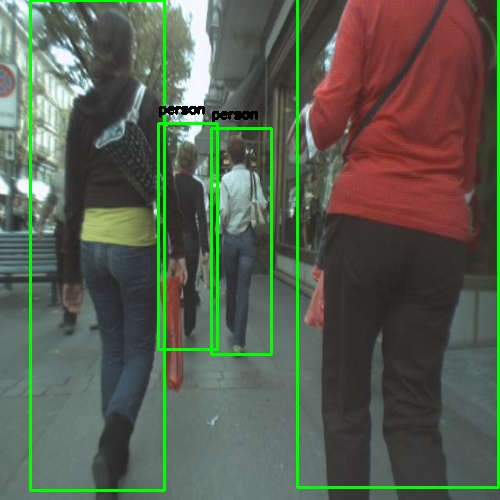
\includegraphics[scale=0.25]{figures/659.jpg}
\caption{Medianflow multiobject tracking on MOT17-05 (selected frames are not sequential)}
\label{fig:medianflow_images}
\end{center}
\end{figure}
\subsection{GOTURN tracking}
The GOTURN (\textit{Generic Object Tracking Using Regression Networks}) is a deep learning based tracking algorithm which learns the motion of the object in an \textit{offline} manner. Many real-time trackers rely on \textit{online} learning that is usually much faster than a deep learning based tracking solution. The authors claim in the original paper \cite{held2016learning} that their system is ``the first neural-network tracker that learns to track generic objects at 100 FPS" (using GPU acceleration, Nvidia GTX 680). However, when using only a CPU the tracker runs at 2,7 FPS according to the authors. This was the main reason to discard this tracker for the project. 
\section{Experimental validation of the final solution}\label{final_sol}
After the unit test experiments, the dl-objecttracker application follows this configuration:
\begin{enumerate}
    \item Neural network: Faster R-CNN InceptionV2, image input size 400x400, confidence threshold 0,5
    \item Tracker: MedianFlow using tracking confidence
\end{enumerate}
Given this configuration, the whole application was evaluated on the complete train set of MOT17Det to obtain the results of our final solution.
\begin{table}[H]
\begin{center}
\begin{tabular}{|c|c|c|c|}
\hline
\textbf{dl\_objecttracker} & \textbf{AP @ 0,5 (\%)} & \textbf{FPS Net} & \multicolumn{1}{l|}{\textbf{FPS Tracker}} \\ \hline
\textbf{MOT17-02}          & 11,59                  & 0,93             & 31,4                                      \\ \hline
\textbf{MOT17-04}          & 17,25                  & 0,869            & 23,96                                     \\ \hline
\textbf{MOT17-05}          & 36,53                  & 0,98             & 37,28                                     \\ \hline
\textbf{MOT17-09}          & 43,53                  & 0,95             & 35,83                                     \\ \hline
\textbf{MOT17-10}          & 23,26                  & 0,943            & 36,18                                     \\ \hline
\textbf{MOT17-11}          & 35,74                  & 0,96             & 41,56                                     \\ \hline
\textbf{MOT17-13}          & 14,04                  & 0,941            & 42,01                                     \\ \hline
\end{tabular}
\end{center}
\caption{Final results on MOT17Det train set}
\label{tab:final}
\end{table}
The best results in terms of average precision occur in the MOT17-09 sequence, followed by MOT17-11 and MOT17-05. This may indicate that the procedure used influences the results giving the better scores in the sequences used to evaluate the performance of the Tracker and Network module. However, from table \ref{tab:annex_2} and table \ref{tab:annex_3} it can be observed that the three mentioned sequences have in common that they have a small number of total ground truth ocurrences. It can be easier for the developed system to get good results in this type of sequences. The results indicate that the developed application performs best on sequences with lowly crowded densities.\\
Refering to the speed of the developed application, the object detection in the neural network is returned with a stable frame rate of about 1 FPS and the tracker runs above 20 FPS in every sequence.